\section{Entendimiento del Negocio y los Datos}
Siguiendo la metodología seleccionada para estructurar este trabajo de minería de datos, la primera etapa de Crisp-DM es la comprensión del negocio y posterior a eso, comprensión de los datos. Esto es lo que se abordará en este apartado, dando a conocer de forma breve los objetivos y requerimientos y luego ahondar en los datos obtenidos. 

Con respecto entendimiento del negocio, tal como es mencionado con profundidad en el Capítulo~\ref{ch:intro}, la finalidad es crear un prototipo de un sistema que permita, en base a información histórica, identificar en tiempo real aquellos estudiantes con riesgo de desertar del sistema escolar o algún foco de deserción escolar. Esto ayudará a a los encargados del diseño y desarrollo de políticas públicas para poder medir el impacto de estas sobre el sistema educativo.

Los requerimientos para poder llevar esto es principalmente la información histórica que se tenga del sistema escolar que será posible manipular gracias a la utilización de herramientas de minería de datos.

\subsection{Fuentes de Información}
En este apartado se presentan las fuentes de información que proveerán datos que respaldarán el desarrollo del modelo de predicción. Previo a esto, es necesario tener claridad de qué información contienen, cómo se obtienen estos datos y sus disponibilidades, para luego definir qué se utilizará y qué no. %Además de cómo se pre-procesará toda esta información, con el fin de evitar errores y datos anómalos. 

Las diferentes entidades del sistema educativo chileno y grupos de investigadores dedicados a la educación preparan y desarrollan diferentes fuentes de información que serán cruciales para el desarrollo de este proyecto, a las que fue posible acceder gracias a la Ley de Transparencia mencionada en el Capítulo~\ref{ch:intro}. 

Nuestras fuentes de información son seis y se detallan a continuación. 

\subsubsection{Centro de estudios del MINEDUC}
El Ministerio de Educación de Chile cuenta con este centro de estudios que tiene como objetivo generar y difundir información relativa a la educación en nuestro país, de donde fue posible obtener las siguientes bases de datos:
\begin{enumerate}
\item Rendimiento anual de los alumnos
\item Matrículas anuales de los alumnos
\item Dotación docente de los establecimientos
\item Información anual de la subvención escolar preferencial
\item Información del SEP
\item Directorio de establecimientos
\item Matrículas de los establecimientos
\item Información anual de los docentes
\item Información anual de la dotación docente
\end{enumerate}

Estas se encuentran disponibles desde el año 2002 hasta el 2014, y la forma en que se obtiene toda esta información es gracias a las diferentes fuentes primarias que se presentan inmediatamente. 

\begin{longdescription}
\item [Sistema de Información General de Estudiantes] \hfill \\
    El Sistema de Información General de Estudiantes, SIGE, es una plataforma web creada por el Ministerio de Educación de Chile que tiene como objetivo integrar en un solo lugar toda la información referente a sostenedores, establecimientos educacionales, docentes y alumnos. 
    
    En este sistema participan todo tipo de establecimientos; municipales, particulares subvencionados y particulares pagados con el fin de hacer llegar la información constantemente. 
    Esta información integra procesos asociados, tales como:
    \begin{itemize}
        \item Matrícula inicial
        \item Declaración de Asistencia
        \item Actas de rendimiento 
        \item Idoneidad docente
        \item Rendimiento 
        \item Ingreso de Asistencia
    \end{itemize}
\item [Sistema de Idoneidad Docente] \hfill \\
    El Sistema de Idoneidad Docente, SIDOC, corresponde a la sistematización de la información relativa al cuerpo docente en ejercicio profesional en cada establecimiento educacional del país. Es un registro censal y anual del Ministerio de Educación de Chile, que consiste en una plataforma implementada a partir del año 2003 y que incluye información de los años 2003 a 2010, ya que del año 2011 en adelante es el SIGE quien proporciona estos datos.
    
    La información que contiene este sistema es: género, edad, título y mención, función que realiza en el establecimiento, nivel y asignatura que realiza cada docente aula, horas y tipo de contrato. A su vez, contiene información respecto a los asistentes de la educación, es decir, sobre los auxiliares, administrativos, y otros profesionales no docentes del establecimiento. 
\item [Registro de Estudiantes de Chile] \hfill \\
    El Registro de Estudiantes de Chile, RECH, es un sistema de información extranet que captura, almacena y administra datos personales y académicos de cada uno de los estudiantes de enseñanza básica y media del país. 
    
    Surge entre los años 2001 y 2002 con el fin de automatizar, normalizar, organizar y mantener una gran base de datos del sistema escolar para generar información de calidad para posteriores estudios, investigaciones y servicios propios del MINEDUC y de otros actores.
    
    Este sistema contiene información relativa a los estudiantes desde el año 2002, y estos datos comprenden principalmente: 
    \begin{itemize}
        \item Identificación del estudiante (RUN)
        \item Establecimiento educacional en que se educa
        \item Plan de estudio que recibe
        \item Equipo docente responsable
        \item Desempeño académico alcanzado
    \end{itemize}
    Existen dos procesos que alimentan con información a este sistema, que exigen la participación de todos los establecimientos educacionales del país oficialmente reconocidos y de todos los sectores (públicos y privados). Estos son:
    \begin{enumerate}
        \item Matrícula inicial: consiste en la captura de información al inicio de cada año escolar, de todos y cada uno de los grados y establecimientos del país. Esta información se registra al 30 de abril, contiene datos personales de cada alumno (nombre, RUN, apellidos, fecha de nacimiento y comuna de residencia) y datos sobre el establecimiento educacional asociado al alumno como su modalidad de enseñanza y curso.
        \item Rendimiento escolar: se trata de la captura de información al final de cada año escolar, de todos y cada uno de los grados y establecimientos del país.Se recogen los datos sobre el plan de estudio o malla curricular, el cuerpo docente por asignatura y el rendimiento académico del alumno ( lo que incluye nota final de cada asignatura, promedio final, \% de asistencia, observaciones y situación final de promoción que puede ser retirado, promovido o reprobado).
    \end{enumerate}
\item [Centro de Perfeccionamiento, Experimentación e Investigaciones Pedagógicas] \hfill \\
    El Centro de Perfeccionamiento, Experimentación e Investigaciones Pedagógicas, CPEIP, es el organismo del Ministerio de Educación encargado de diseñar, implementar y evaluar todo lo referente a los docentes, equipos directivos y asistentes de la educación.
    
    El CPEIP es responsable de llevar un Registro Público Nacional de Perfeccionamiento de todos los cursos que se ofrecen a los profesores dependientes del sector municipal, con el fin que puedan impetrar el reconocimiento y pago de la Asignación de Perfeccionamiento.
    
    En este registro, se inscriben cursos realizados por el CPEIP, por las Instituciones de Educación Superior autónomas y por las Instituciones Públicas o Privadas debidamente acreditadas por el CPEIP.
    
    Además tiene la obligación de difundir los cursos inscritos de manera que los profesores tengan información para escoger adecuadamente el curso que les interesa profesionalmente y los municipios puedan verificar la real existencia de los cursos nominados en los certificados que le entregan los profesionales de la educación de su dependencia.
\end{longdescription}

\subsection{Agencia de Calidad}
La Agencia de Calidad, mencionada en el apartado 1.1.3 del Capítulo 1 del presente documento, es el encargado del SIMCE y de toda la información que de esta prueba se obtiene. 

Dentro de sus registros, se genera información a tres niveles diferentes: 
\begin{itemize}
\item Estudiantes: dan origen a información de dos índoles; por un lado se obtienen los resultados de las pruebas SIMCE, con sus puntajes, y por otro lado se obtienen los resultados de cuestionarios aplicados a los mismos estudiantes evaluados, en los que se indaga sobre aspectos generales de su establecimiento escolar, así como sobre sus procesos y estrategias de aprendizaje dentro y fuera del aula, sus intereses y motivaciones, entre otros temas.
\item Docentes: resultados de cuestionarios respondidos por los profesores de cada curso evaluado y contienen preguntas relativas a su formación profesional y a los contenidos que enseñó durante el año escolar, entre otros aspectos.
\item Apoderados: resultados de cuestionarios respondidos por los apoderados de cada estudiante evaluado, donde se indaga sobre el nivel educacional de los padres, ingreso del hogar y nivel de satisfacción con el establecimiento, entre otros.
\end{itemize}

A partir de toda esta información, se obtienen las siguientes bases de datos:
\begin{enumerate}
\item Encuesta SIMCE
\item Otros indicadores de la calidad de la educación (OIC)
\end{enumerate}

La disponibilidad de la Encuesta SIMCE es desde el año 1998 hasta el 2014, mientras que los OIC se encuentran disponibles sólo a partir del año 2010 y hasta el año 2014. 

\subsection{Más Información Mejor Educación}
Más Información Mejor Educación, o MIME\footnote{Para mayor información, revisar la página web http://www.mime.mineduc.cl}, es una página web perteneciente al Ministerio de Educación en la cual se puede acceder a información relevante de todos los establecimientos educacionales de Chile, sean estos municipales, particulares subvencionados o particulares pagados. 
La información a la cual se puede acceder es:
\begin{itemize}
\item Descripción de la Escuela
\item Proyectos Educativos
\item Contactos
\item Resultados Simce y PSU
\item Evaluación Docente
\item Procesos de Selección
\item Mensualidad y Matrícula
\item Mapa Comunal
\end{itemize}

Específicamente, las bases de datos obtenidas de esta fuente, y con las que se trabajarán, son las siguientes: 
\begin{enumerate}
\item Becas escolares disponibles
\item Matrícula total
\item Promedio PSU del año 2013
\item Indicador de la gestión tecnológica
\item Indicador del uso de la infraestructura tecnológica
\item Vacantes en el curso de entrada
\item Promedio de alumnos por curso
\end{enumerate}


\subsection{Junta Nacional de Auxilio Escolar y Becas}
La Junta Nacional de Auxilio Escolar y Becas, JUNAEB, también actúa como una fuente de información, aportando con el indicador IVE-SINAE. Este permite medir la condición de vulnerabilidad de todos los alumnos, y se construye con insumos de diferentes fuentes de información de cada estudiante y que llegan a JUNAEB mediante convenios interinstitucionales, como encuestas de vulnerabilidad JUNAEB, sistema de afiliación de salud, pertenecer a algún programa de la red SENAME, entre otros. 

\begin{enumerate}
\item Índice de vulnerabilidad por establecimiento
\item Índice de vulnerabilidad escolar promedio
\end{enumerate}

\begin{longdescription}
\item [Unidad de Apoyo Municipal] \hfill \\
La Unidad de Apoyo Municipal, UNAM, fue creado en el año 2010 y es el representante del Ministerio de Educación frente a las relaciones con las municipalidades, en los aspectos de gestión, prestando asesoría a quienes lo requieran con el fin de generar alternativas eficaces de mejora en la gestión administrativa, financiera y técnica del área de educación de cada municipio.
En la UNAM existen dos áreas de trabajos, una de ellas está dedicada a la administración de programas específicos para municipios, como el Fondo de Apoyo a la Gestión, FAGEM, el Bono al Retiro Docente, el Fondo para Docentes Jubilados, Fondos Municipales de Gestión, el Fondo de Reconversión, el Sistema Nacional de Evaluación del Desempeño, SNED, y en general las transferencias de recursos.  
Con respecto a este último, el Sistema Nacional de Evaluación del Desempeño, son los encargados de proveer la información referente al desempeño de los profesionales de la educación. 
\end{longdescription}

\subsection{Centro de Investigación Avanzada en Educación}
Como fue mencionado anteriormente en el Capítulo~\ref{ch:intro}, el CIAE es una entidad dedicada a la investigación en el área de la educación, y en base a esto y a la información que tienen acceso, han ido generando algunas bases de datos como:

\begin{enumerate}
\item Distancias a establecimiento
\item Profesores taxi
\end{enumerate}

\subsection{Centro de Inteligencia Territorial}
El Centro de Inteligencia Territorial, CIT, de la Universidad Adolfo Ibáñez es el encargado de generar bases de datos geolocalizados de alta calidad mediante la incorporación de nuevas tecnologías y gracias a la colaboración de diversas entidades. 

Dentro de la información que reúnen, almacenan y gestionan, está el grupo socioeconómico, niveles de delincuencia, cantidades de áreas verdes, cultura, usos de suelo, entre otros. Toda esta información se encuentra geolocalizada y definida mediante isócronas\footnote{Una isócrona es un área geométrica en un mapa que muestra individuos con una misma característica, como por ejemplo misma manzana}, por lo que permite conocer estas características en diferentes sectores del país.

La base de datos que reúne toda esta información es:
\begin{enumerate}
\item Indicadores territoriales
\end{enumerate}

Se encuentra disponible para el año 2013. 

%Al ver disponibilidad de bases de datos, podemos destacar y mencionar que, asegurando la calidad de estas fuentes de información y la creación de diferentes indicadores relevantes que indiquen deserción escolar, es posible desarrollar una herramientas potente, pues se tiene información de el rendimiento, asistencia, características socio-económicas familiares de estudiantes, junto con caracterizaciones de vulnerabilidad, delitos y ambiente de las diferentes comunas, e inclusive isócronas\footnote{Una isócrona es un área geométrica en un mapa que muestra individuos con una misma característica, como por ejemplo misma manzana} de la manzana del colegio y/o estudiante.
 %   \includepdf[pages={1},trim=0cm 5cm 0cm 0cm]{Figuras/6SolucionPropuesta/Exploracion.pdf}
\begin{figure}[H]
  \centering
    \includegraphics[page=2,angle=90,trim=0 0 100 0,scale=0.7]{Figuras/6SolucionPropuesta/eexploracion.pdf}
      \caption{Distribución de la tasa de deserción por la edad del alumno agrupado por genero}
    \label{fig:tdea}
\end{figure}